\documentclass[../main.tex]{subfiles}
\begin{document}
\section{Introduction}
\label{sec:intro}
\begin{figure}[H]
    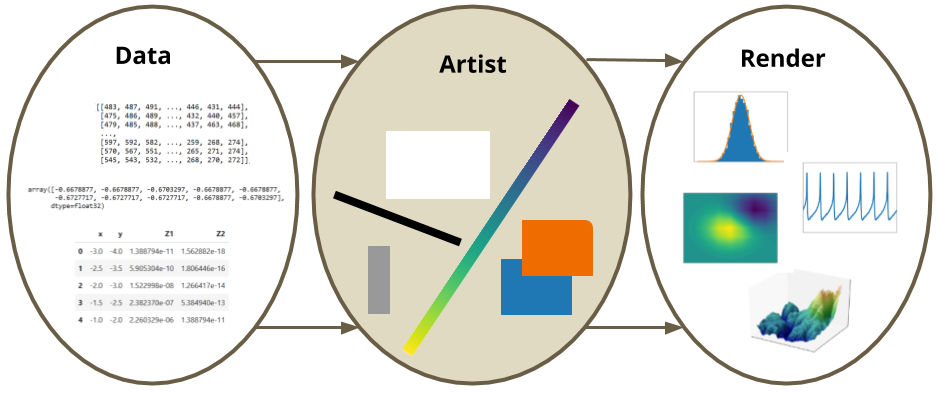
\includegraphics[width=\textwidth]{figures/intro/dar.png}
    \caption{Visualization is a mapping from data into visual encodings that are then rendered into images. In our model, this visual encoding stage is called the artist.}
    \label{fig:intro_artist_stages}
\end{figure}
The work presented in this paper is motivated by a need for a library of visualization components that developers could use to build complex, domain specific tools tuned to the semantics and structure carried in domain specific data. While many researchers have identified and described important aspects of visualization, they have specialized in such different ways as to not provide a model general enough to natively support the full range of data and visualization types many general purpose modern visualization tools may need to support. The core architecture also needs to be robust to the big data needs of many visualization practitioners, and therefore support distributed and streaming data needs. To support both exploratory and confirmatory visualization\cite{tukeyWeNeedBoth1980}, this tool needs to support 2D and 3D, static, dynamic and interactive visualizations. 

Specifically, this work was driven by a rearchitecture of the Python visualization library Matplotlib\cite{hunterMatplotlib2DGraphics2007} to meet modern data visualization needs. We aim to take advantage of developments in software design, data structures, and visualization to improve the consistency, composibility, and discoverability of the API. To do so, this work first presents a mathematical description of how data is transformed into graphic representations, as shown in figure~\ref{fig:intro_artist_stages}. As with other mathematical formalisms of visualization \cite{mackinlayAutomatingDesignGraphical1986,kindlmann2014algebraic,sugibuchiFramwork2009,vickersUnderstandingViz2013}, a mathematical framework provides a way to formalize the properties and structure of the visualization. In contrast to the other formalisms, the model presented here is focused on the components that build a visualization rather than the visualization itself. 

In other words this model is not intended to be evaluative, it is intended to be a reference specification for visualization library API. To make this model as implementation independent as possible, we propose fairly general mathematical abstractions of the data container such that we do not need to assume the data has any specific structure, such as a relational database. We reuse this structure for the graphic as that allows us to specifically discuss how structure is preserved. We take a functional approach because functional paradigms encourage writing APIs that are flexible, concise and predictable due to the lack of side effects \cite{loudenProgrammingLanguagesPrinciples2010}. Furthermore, by structuring the API in terms of composition of the smallest units of transformation for which we can define correctness, a functional paradigm naturally leads to a library of highly modular components that are composable in such a way that by definition the composition is also correct. This allows us to ensure that domain specific visualizations built on top of these components are also correct without needing knowledge of the domain. As with the other mathematical formalisms of visualization, we factor out the rendering into a separate stage; but, our framework describes how these rendering instructions are generated. 

In this work, we present a framework for understanding visualization as equivariant maps between topological spaces. Using this mathematical formalism, we can interpret and extend prior work and also develop new tools. We validate our model by using it to re-design artist and data access layer of Matplotlib, a general purpose visualization tool.
 

\section{Background}
One of the reasons we developed a new formalism rather than adopting the architecture of an existing library is that most information visualization software design patterns, as categorized by Heer and Agrawala\cite{HeerSoftware2006}, are tuned to very specific data structures. This in turn restricts the design space of visual algorithms that display information (the visualization types the library supports) since the algorithms are designed such that the structure of data is assumed, as described in Tory and Möller's taxonomy \cite{ToryRethinkingVisualization2004}. In proposing a new architecture, we contrast the trade offs libraries make, describe different types of data continuity, and discuss metrics by which a visualization library is traditionally evaluated. 

\subsection{Tools}
\label{sec:intro_data_tools}
One extensive family of relational table based libraries are those based on Wilkenson's Grammar of Graphics (GoG) \cite{wilkinsonGrammarGraphics2005}, including ggplot\cite{wickhamGgplot2ElegantGraphics2016a}, protovis\cite{bostockProtoviz2009} and D3 \cite{bostockDataDrivenDocuments2011}, vega\cite{satyanarayanDeclarativeInteractionDesign2014} and altair\cite{vanderplasAltairInteractiveStatistical2018}. The restriction to tables in turn restricts the native design space to visualizations suited to tables. Since the data space and graphic space is very well defined in this grammar, it lends itself to a declarative interface \cite{heerDeclarative2010}. This grammar oriented approach allows users to describe how to compose visual elements into a graphical design \cite{wongsuphasawatNavigatingWideWorld2021}, while we are proposing a framework for building those elements. An example of this distinction is that the GoG grammar includes computation and aggregation of the table as part of the grammar, while we propose that most computations are specific to domains and only try to describe them when they are specifically part of the visual encoding - for example mapping data to a color. Disentangling the computation from the visual transforms allows us to determine whether the visualization library needs to handle them or if they can be more efficiently computed by the data container.


A different class of user facing tools are those that support images, such as ImageJ\cite{schneiderNIHImageImageJ2012} or Napari\cite{nicholas_sofroniew_2021_4533308}. These tools often have some support for visualizing non image components of a complex data set, but mostly in service to the image being visualized. These tools are ill suited for general purpose libraries that need to support data other than images because the architecture is oriented towards building plugins into the existing system \cite{WritingPlugins} where the image is the core data structure. Even the digital humanities oriented ImageJ macro ImagePlot\cite{studiesCulturevisImageplot2021}, which supports some non-image aggregate reporting charts, is still built around image data as the primary input. 

There are also visualization tools where there is no single core structure, and instead internally carry around many different representations of data. Matplotlib, has this structure, as does VTK \cite{hanwellVisualizationToolkitVTK2015,geveci2012vtk} and its derivatives such as MayaVi\cite{RamachandranMayaVI2011} and extensions such as ParaView\cite{ahrens2005paraview} and the infoviz themed Titan\cite{brianwylieUnifiedToolkitInformation2009}. Where GoG and ImageJ type libraries have very consistent APIs for their visualization tools because the data structure is the same, the APIs for visualizations in VTK and Matplotlib are significantly dependent on the structure of the data it expects. This in turn means that every new type of visualization must carry implicit assumptions about data structure in how it interfaces with the input data. This has lead to poor API consistency and brittle code as every visualization type has a very different point of view on how the data is structured. This API choice particularly breaks down when the same dataset is fed into visualizations with different assumptions about structure or into a dashboard consisting of different types of visualization\cite{a.sarikayaWhatWeTalk2019,fewDashboardConfusionRevisited2007} because there is no consistent way to update the data and therefore no consistent way of guaranteeing that the views stay in sync. Our model is a structure dependent formalism, but then also provides a core representation of that structure that is abstract enough to provide a common interface for many different types of visualization.

\subsection{Data}
\label{sec:intro_data}
Discrete and continuous data and their attributes form a discipline independent design space \cite{pousmanCasualInformation2007}, so one of the drivers of this work was to facilitate building libraries that could natively support domain specific data containers that do not make assumptions about data continuity. As shown in figure~\ref{fig:intro_data_format}, there are many types of connectivity. A database typically consists of unconnected records, while an image is an implicit 2D grid and a network is some sort of explicitly connected graph. These data structures typically contain not only the measurements or values of the data, but also domain specific semantic information such as that the data is a map or an image that a modern visualization library could exploit if this information was exposed to the API. 

\begin{figure}[H]
    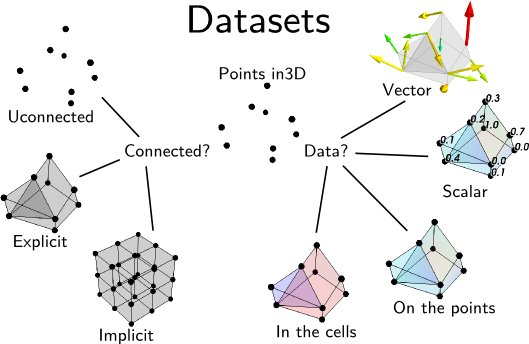
\includegraphics[width=1\textwidth]{figures/intro/dataset_diagram.png}
    \caption{One way to describe data is by the connectivity of the points in the dataset. A database for example is often discrete unconnected points, while an image is an implicitely connected 2D grid. This image is from the Data Representation chapter of the MayaVi 4.7.2 documentation.\cite{DataRepresentationMayavi}}
    \label{fig:intro_data_format}
\end{figure}
As shown in figure~\ref{fig:intro_data_format}, there are many distinct ways of encoding each specific type of structure, while as mentioned in section~\ref{sec:intro_data_tools} APIs are clearer when structured around a common data representation. Fiber bundles were proposed by Butler as one such representation because they encode the continuity of the data separately from the types of variables and are flexible enough to support discrete and ND continuous datasets \cite{butlerVisualizationModelBased1989,butlerVectorBundleClassesForm1992}. Since Butler's model lacks a robust way of describing variables, we fold in Spivak's Simplicial formulation of databases \cite{spivakDatabasesAreCategories2010,spivakSIMPLICIALDATABASES} so that we can encode a schema like description of the data in the fiber bundle. In this work we will refer to the points of the dataset as \textit{records} to indicate that a point can be a vector of heterogenous elements. Each \textit{component} of the record is a single object, such as a temperature measurement, a color value, or an image. We also generalize \textit{component} to mean all objects in the dataset of a given type, such as all temperatures or colors or images. The way in which these records are connected is the \textit{connectivity}, \textit{continuity}, or more generally \textit{topology}.

\begin{mdframed}[roundcorner=10pt, frametitle= definitions, frametitlerule=true, frametitlebackgroundcolor=gray!10]
    \begin{description}
        \item[\textbf{records}] points, observations, entries 
        \item[\textbf{components}] variables, attributes, fields 
        \item[\textbf{connectivity}] how the records are connected to each other
    \end{description}
\end{mdframed}

Often this topology has metadata associated with it, describing for example when or where the measurement was taken. Building on the idea of metadata as \textit{keys} and their associated \textit{values} proposed by Munzner \cite{munznerChDataAbstraction}, we propose that information rich metadata are part of the components and instead the values are keyed on coordinate free structural ids. In contrast to Munzner's model where the semantic meaning of the key is tightly coupled to the position of the value in the dataset, our model considers keys to be a pure reference to topology. This allows the metadata to be altered, for example by changing the coordinate systems or time resolution, without imposing new semantics on the underlying structure.

\subsection{Visualization}
\label{sec:intro_viz}
\begin{figure}[H]
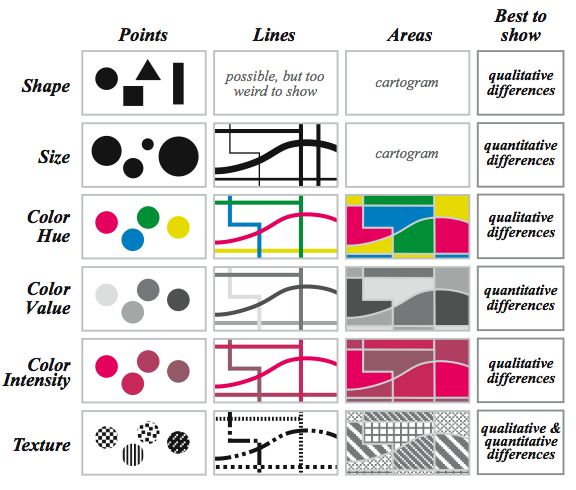
\includegraphics[width=1\textwidth]{figures/intro/retinal_variables.png}
\caption{Retinal variables are a codification of how position, size, shape, color and texture are used to illustrate variations in the components of a visualization. The best to show column describes which types of information can be expressed in the corresponding visual encoding. This tabular form of Bertin's retinal variables is from Understanding Graphics \cite{malamedInformationDisplayTips2010} who reproduced it from Krygier and Wood's \textit{Making Maps: A Visual Guide to Map Design for GIS} 
\cite{krygierMakingMapsVisual2005}}
\label{fig:intro_retinal_variables}
\end{figure}

Visual representations of data, by definition, reflect something of the underlying structure and semantics\cite{friendlyBriefHistoryData2008}, whether through direct mappings from data into visual elements or via figurative representations that have meaning due to their similarity in shape to external concepts \cite{byrneAcquiredCodesMeaning2016}. The components of a visual representation were first codified by Bertin\cite{bertinSemiologyGraphicsDiagrams2011a}.  As illustrated in figure~\ref{fig:intro_retinal_variables}, Bertin proposes that there are classes of visual encodings such as shape, color, and texture that when mapped to from specific types of measurement, quantitative or qualitative, will preserve the properties of that measurment type. For example, that nominal data mapped to hue preserves the selectivity of the nominal measurements. Furthermore he proposes that the visual encodings be composited into graphical marks that match the connectivity of the data - for example discrete data is a point, 1D continuous is the line, and 2D data is the area mark. A general form of marks are glyphs, which are graphical objects that convey one or more attributes of the data entity mapped to it\cite{ware2019information, munznerVisualizationAnalysisDesign2014} and minimally need to be differentiable from other visual elements \cite{ziemkiewiczEmbeddingInformationVisualization2009}. The set of encoding relations from data to visual representation is termed the graphical design by Mackinlay \cite{mackinlayAutomatingDesignGraphical1986, mackinlayAUTOMATICDESIGNGRAPHICAL1987} and the design rendered in an idealized abstract space is what throughout this paper we will refer to as a graphic. 

The measure of how much of the structure of the data the graphic encodes is a concept Mackinlay termed expressiveness, while the graphic's effectiveness describes how much design choices are made in deference to perceptual saliency \cite{clevelandResearchStatisticalGraphics1987,clevelandGraphicalPerceptionTheory1984,chambersGraphicalMethodsData1983a, munznerVisualizationAnalysisDesign2014}. When the proporties of the representation match the properties of the data, then the visualization is easier to understand according to Norman's Naturalness Principal\cite{NaturalnessPrincipleInfoVis}. These ideas are combined into Tufte's notion of graphical integrity, which is that a visual representation of quantitative data must be directly proportional to the numerical quantities it represents (Lie Principal), must have the same number of visual dimensions as the data, and should be well labeled and contextualized, and not have any extraneous visual elements \cite{tufteVisualDisplayQuantitative2001}. This notion of matching is explictely formalized by Mackinlay as a structure preserving mapping of a binary operator from one domain to another \cite{mackinlayAUTOMATICDESIGNGRAPHICAL1987}. A functional dependency framework for evaluating visualizations was proposed by Sugibuchi et al \cite{sugibuchiFramwork2009}, and an algebraic basis for visualization design and evaluation was proposed by Kindlmann and Scheideggar\cite{kindlmann2014algebraic}. Vickers et al. propose a category theory framework\cite{vickersUnderstandingViz2013} that extends structural preservation to layout, but is focused strictly on the design layer like the other mathematical frameworks.

\begin{figure}[H]
    \begin{subfigure}{.24\textwidth}
        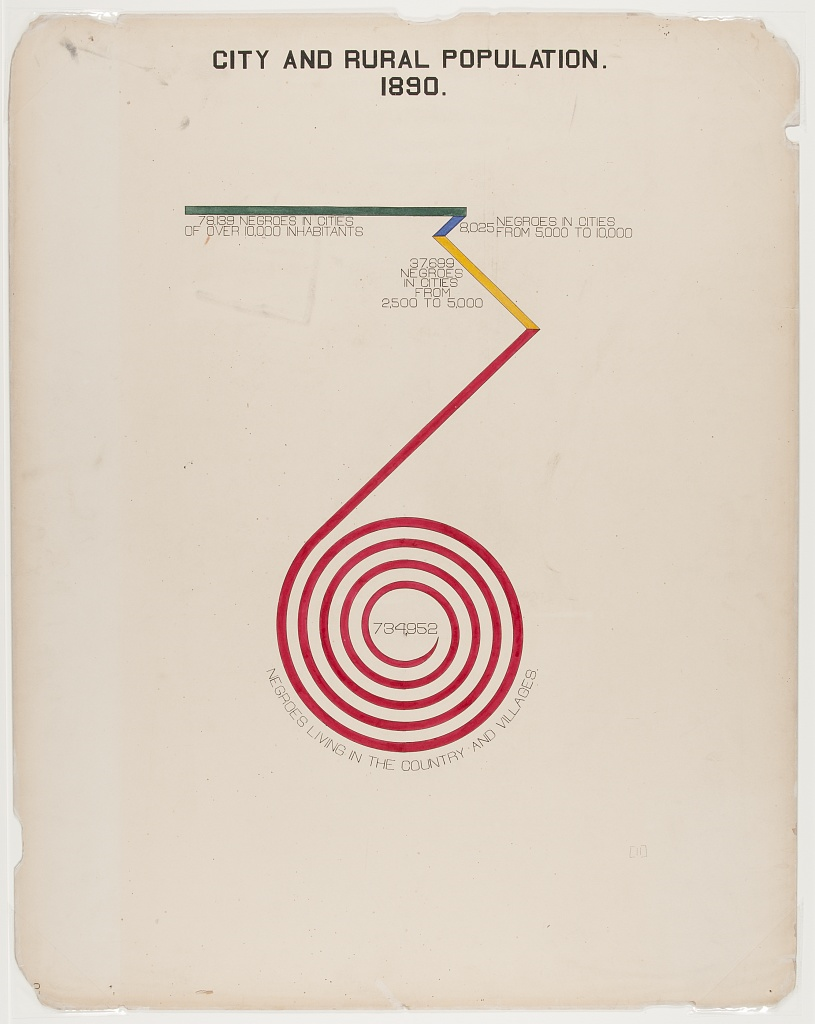
\includegraphics[width=1\textwidth]{figures/intro/du_bois_spinny.png}
        \caption{}
        \label{fig:intro_dpa}
    \end{subfigure}
    \begin{subfigure}{.24\textwidth}
        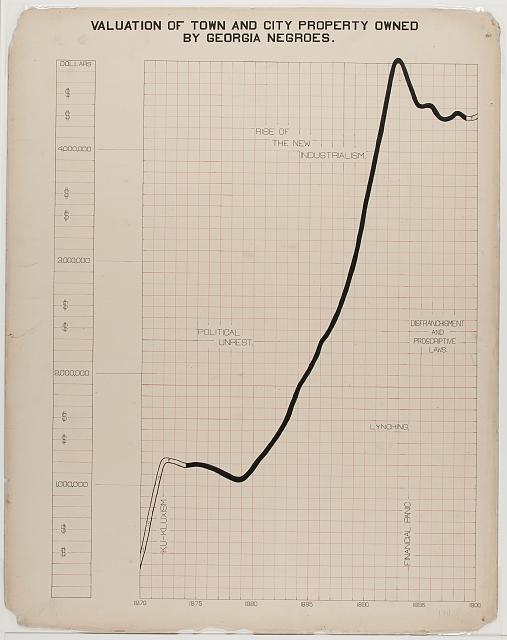
\includegraphics[width=1\textwidth]{figures/intro/du_bois_line.png}
        \caption{}
        \label{fig:intro_dpb}
    \end{subfigure}
    \begin{subfigure}{.24\textwidth}
        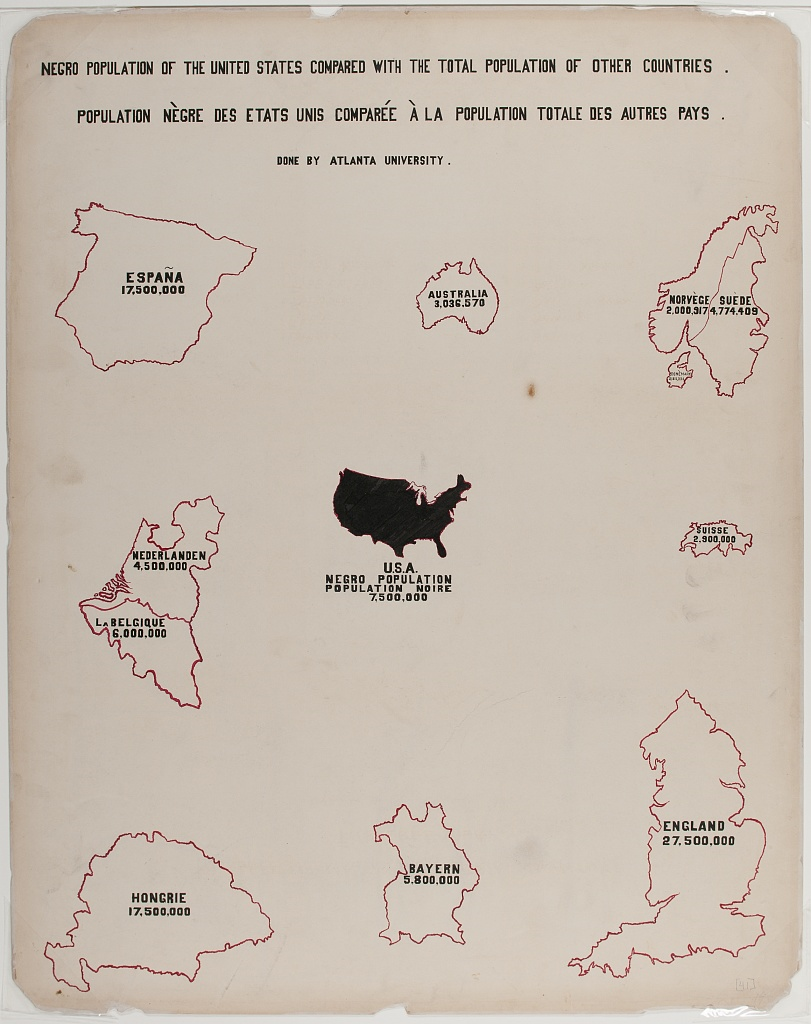
\includegraphics[width=1\textwidth]{figures/intro/du_bois_country.png}
        \caption{}
        \label{fig:intro_dbc}
    \end{subfigure}
    \begin{subfigure}{.24\textwidth}
        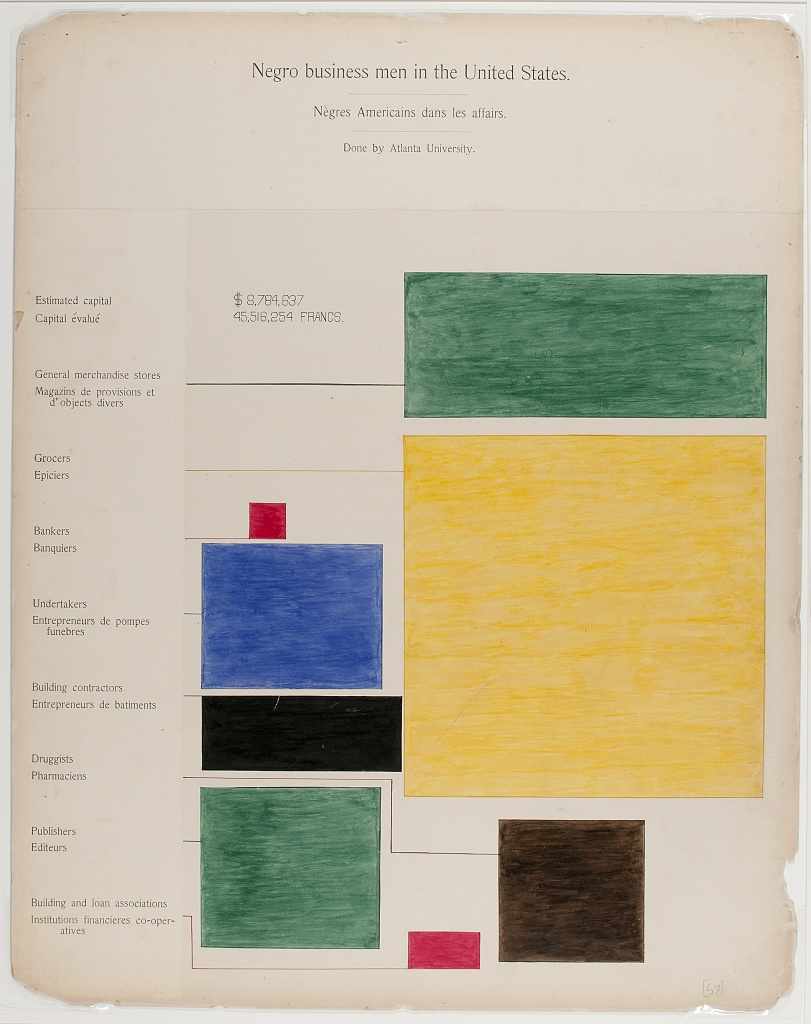
\includegraphics[width=1\textwidth]{figures/intro/du_bois_heat.png}
        \caption{}
        \label{fig:intro_dbd}
    \end{subfigure}
    \caption{Du Bois' data portraits\cite{duboiscenterattheuniversityofmassachusettsBoisDataPortraits2018} of post reconstruction Black American life exemplify that the fundemental characteristics of data visualization is that the visual elements vary in proportion to the source data. In figure~\ref{fig:intro_dpa}, the length of each segment maps to population; in figure~\ref{fig:intro_dpb}, the line changes color to indicate a shift in the political environment; in figure~\ref{fig:intro_dbc} the countries are scaled to population size; and figure~\ref{fig:intro_dbd} is a treemap where the area of the rectangle is representative of the number of businesses in each field. The images here are from the Prints and Photographs collection of the Library of Congress \cite{duboisGeorgiaNegroCity1900,duboisGeorgiaNegroValuation1900, duboisSeriesStatisticalCharts, duboisSeriesStatisticalChartsa}}
    \label{fig:intro_dubois}
\end{figure}

One example of highly expressive visualizations are the data portraits by Du Bois shown in figure~\ref{fig:intro_dubois}. While the Du Bois charts are different from the usual scatter, line, and plot charts, they conform to the constraint that a graphic is a structure preserving map from data to visual representation. Figure~\ref{fig:intro_dpa} is semantically similar to a bar chart in that the lengths of the segments are mapped to the values, but in this chart the segments are stacked together. Figure~\ref{fig:intro_dpb} is a multicolored line chart where the color shifts are at periods of political significance. In figure~\ref{fig:intro_dbc}, Du Bois combines a graphical representation where glyph size varies by population with a figurative representation of those glyphs as the countries the data is from, which means that the semantic and numerical properties of the data are preserved in the graph. Figure~\ref{fig:intro_dpd} is simply a treemap\cite{heerTourVisualizationZoo2010} with space between the marks. Since the Du Bois data portraits meet the criteria of a faithful visual representation, we propose a mathematical framework and implementation that allows us to express the Du Bois charts and common chart types with equal fidelity. 

\subsection{Contribution}
This work presents a mathematical model of the transformation from data to graphic representation and a proof of concept implementation. Specifically, the contributions of this work are 

\begin{enumerate}
    \item a formal description of the topology preserving relationship between data and graphic via continuous maps
    \item a formal description of the property preservation from data component to visual representation as equivariant maps that carry a homomorphism of monoid actions
    \item abstraction of data as a fiber bundle with schema like fibers to encode components and topology 
    \item algebraic sum operator such that more complex visualizations can be built from simple ones 
    \item a functional oriented visualization tool architecture built on the mathematical model to demonstrate the utility of the model
    \item a prototype of the architecture built on Matplotlib's infrastructure to demonstrate the feasibility of the model
\end{enumerate}

In contrast to mathematical models of visualization that aim to evaluate visualization design, we propose a topological framework for building tools to build visualizations. We defer judgement of expressivity and effectiveness to developers building domain specific tools, but provide them the framework to do so. 
\end{document}